
In this work, we are quantifying the effect of super-sample effect on the covariance matrix of higher-order statistics for a weak lensing survey. To achieve this, we are conducting a series of N-body simulations and analyzing the resulting convergence maps. These maps allow us to compute the statistics and covariance matrices for various statistical measures. Therefore, we can investigate the impact of super-sample covariance on the covariance matrices of these statistics.

In the following sections, we will discuss the methodology used to generate the convergence maps, extract patches for analysis, incorporate noise, apply Gaussian smoothing, and compute the statistical measures. We will also outline the process for estimating the covariance matrices and comparing the results between the BIGBOX and TILED simulations. 

\section{Constructing the BIGBOX and TILED Datasets}
We employed the publicly available particle-mesh simulation code, \texttt{FASTPM} \citep{10.1093/mnras/stw2123} to generate the simulations used in this study. As discussed in Section~\ref{sec:fastpm}, \texttt{FASTPM} is chose to achieve high accuracy while minimizing computational time. 

The two simulations we have used are \textbf{BIGBOX} and \textbf{TILED}. For both simulations, we have used the same cosmological parameters as the IllustrisTNG project \citep{2019ComAC...6....2N}. The parameters are listed in Table~\ref{tab:simulations}. 

\begin{table}[h]
    \centering
    \begin{tabular}{lcc}
    \toprule
    \textbf{Parameter} & \textbf{Symbol} & \textbf{Value} \\
    \midrule
    Hubble constant & $H_0$ & 67.74 \, [$\mathrm{km\,s^{-1}\,Mpc^{-1}}$] \\ 
    Matter density & $\Omega_m$ & 0.3089 \\
    Baryon density & $\Omega_b$ & 0.0486 \\
    Amplitude of fluctuations & $\sigma_8$ & 0.8159 \\
    Spectral index & $n_s$ & 0.9667 \\
    Sum of neutrino masses & $M_{\nu}$ & 0.0 \, [eV] \\
    \bottomrule
    \end{tabular}
    \caption{Cosmological parameters used in the N-body simulations.}\label{tab:simulations}
    \end{table}

The BIGBOX simulation, conducted as part of the HalfDome project \citep{2024arXiv240717462B}, models using $6144^3$ particles, a box with a side length of $3750$ Mpc/h and periodic boundary conditions.
They are replicated aprroximately $2.6$ times per dimension too cover the volume between $z = 0 - 4$, covering about $10$ Gpc/h$^3$ volume.
At the maximum redshift we will consider, $z = 2.5$, the simulation volume is replicated approximately $1.2$ times per dimension.

The TILED simulation covers a smaller volume with side length $L = 625$ Mpc/h, populated with $1024^3$ particles and also with periodic boundary condition. This combination of box size and particle number is chosen to match the resolution of the BIGBOX simulation. To fully cover the same redshift range as the BIGBOX simulation, we replicated the box $10$ times along each axis, though $6$ times is sufficient to cover the volume between $z = 0 - 2.5$. Figure~\ref{fig:simulationsetting} showcases the spatial and redshift setup for the BIGBOX and TILED simulations used in cosmological studies. 

\begin{figure}[ht]
    \centering
    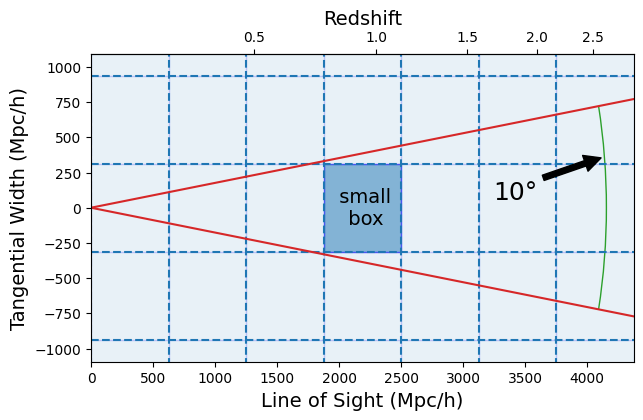
\includegraphics[width=0.8\textwidth]{figures/light_cone_configuration.png}
    \caption[Spatial and redshift setup for the BIGBOX and TILED simulations]{Spatial and redshift setup for the BIGBOX and TILED simulations. Dashed blue grids partition the overall simulation volume into smaller, manageable tiling regions where each tile is a replication of the TILED simulation. The lower horizontal axis represents the line-of-sight distance measured in $\mathrm{Mpc}/h$, with the corresponding redshift values displayed on the top axis.} \label{fig:simulationsetting}
\end{figure}

Both simulations commence at an initial redshift of $z = 9$, utilizing an initial linear matter power spectrum at $z = 0$ generated via the \texttt{CLASS} code \citep{2011JCAP...07..034B}. We evolved the simulations over $60$ time steps, reaching the present day ($z = 0$). The resulting particle distributions are returned in $80$ shells spanning scale factors from $a = 0.2$ to $a = 1.0$ with a uniform spacing of $\Delta a = 0.01$. At each scale factor $a_i$, particles within the shells are projected onto a HEALPix grid \citep{Górski_2005} with $N_{\text{side}} = 8192$, providing an angular resolution of approximately $0.43$ arcminutes, to create mass maps.

The BIGBOX and TILED simulations were executed on the TACC (Texas Advanced Computing Center) cluster. Specifically, the BIGBOX simulations required approximately $4$ hours per realization utilizing $2048$ nodes, while the TILED simulations were completed in $2$ hours per realization utilizing $64$ nodes. 

In total, we obtained $11$ realizations of the BIGBOX simulation and $20$ realizations of the TILED simulation, each initialized with distinct initial seeds. This ensemble of realizations allows us to robustly sample cosmic variance and ensures that our statistical analyses are not biased by any single simulation's initial conditions. 

It is important to note that the observer is positioned at the corner point shared by $8$ replicated boxes for both the TILED and BIGBOX simulations. This placement induces the Box Replication Effect, characterized by a Kaleidoscope pattern of heavily tiled regions along the line of sight and near the equatorial regions (see Figure~\ref{fig:boxreplication_patch} for $z = 1.5$), particularly in directions parallel to the box edges. These replicated regions can introduce artificial correlations and anisotropies in the mass maps, potentially biasing our statistical measurements. To address this, we exclude the most heavily tiled regions from our analysis, ensuring that our results are not significantly impacted by the Box Replication Effect. A detailed discussion of this phenomenon and its implications is provided in Section~\ref{sec:boxreplication}.

\begin{figure}[ht]
    \centering
    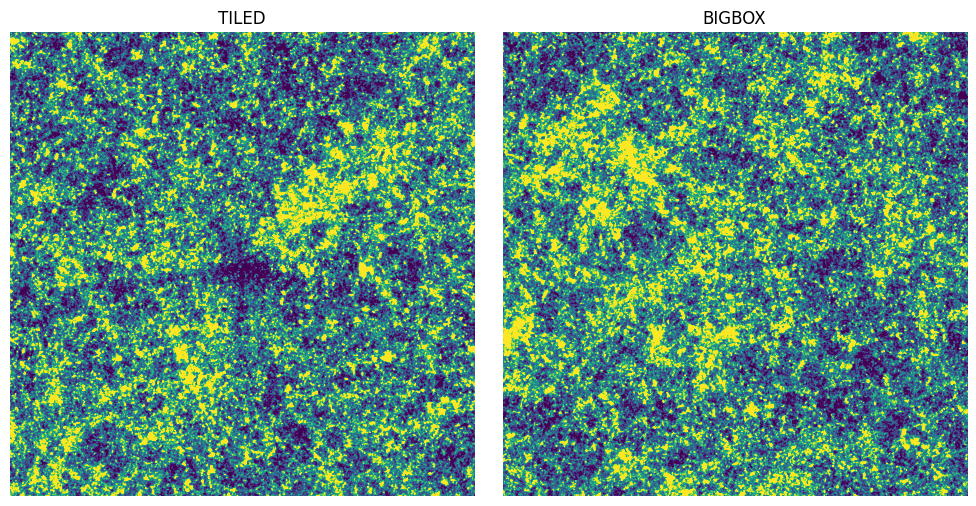
\includegraphics[width=\textwidth]{figures/samplepatch.png}
    \caption[Illustration of a $5 \times 5$ patch at $z = 1.5$]{Illustration of a $5 \times 5$ patch around $(\theta, \phi)= (\pi/2, 0)$ extracted from the TILED and BIGBOX simulations at $z = 1.5$. The TILED simulation exhibits a distinct Kaleidoscope pattern due to box replication, resulting in heavily tiled regions along the line of sight and near the equator. This pattern becomes more pronounced as the redshift increases.}
    \label{fig:boxreplication_patch}
\end{figure}

\section{Producing Weak Lensing Convergence Maps at Multiple Redshifts}
Since we already have the projected mass map at each scale factor, we can calculate the convergence map at each redshift following the discussion in Section~\ref{sec:convergence} and~\ref{sec:weak-lensing-generation}. Since the difference between TILED and BIGBOX simulations due to the super-sample effect shows up at the redshift $z \approx 1$, it is worthful to check the constribution from each redshift to the convergence map.

Figure~\ref{fig:lensing_efficiency} presents the normalized lensing efficiency as a function of the comoving distance (measured in Mpc/$h$) for multiple source redshifts ($z$). The lensing efficiency curves exhibit multiple peaks at intermediate comoving distances, indicating the regions where the distribution of matter along the line of sight most significantly enhances the gravitational lensing signal. 

\begin{figure}
    \centering
    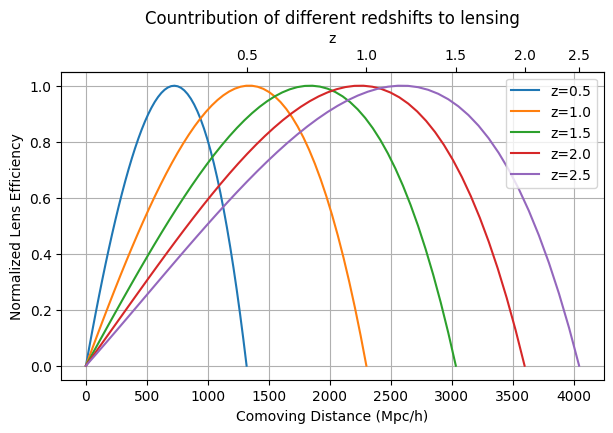
\includegraphics[width=0.8\textwidth]{figures/lensefficiency.png}
    \caption[Normalized lensing efficiency for multiple source redshifts]{Normalized lensing efficiency as a function of comoving distance for multiple source redshifts. The lensing efficiency peaks at intermediate comoving distances, indicating regions where the distribution of matter enhances the gravitational lensing signal.} \label{fig:lensing_efficiency}
\end{figure}

We considered source redshifts $z_s = [0.5, 1.0, 1.5, 2.0, 2.5]$, covering the range of distances that are relevant for both current and upcoming galaxy surveys. At low redshift ($z < 1$), both the BIGBOX and TILED simulations suffer from super-sample effects. However, for higher redshifts ($z > 1$), these effects become more significant in the BIGBOX simulation. This divergence arises because, at approximately $z = 1$, the light cone in the TILED simulation begins to extend tangentially across multiple replicated boxes. Consequently, no additional super-survey modes arise within the TILED simulation beyond this redshift, effectively mitigating the influence of super-sample covariance. 

Figure~\ref{fig:convergence_maps} illustrates the convergence maps generated from both the BIGBOX and TILED simulations at $z_s = 1.5$. Consistent with the methodology employed, these maps are depicted on \textsc{Healpix} grids with $N_{\text{side}} = 8192$.

\begin{figure}
    \centering
    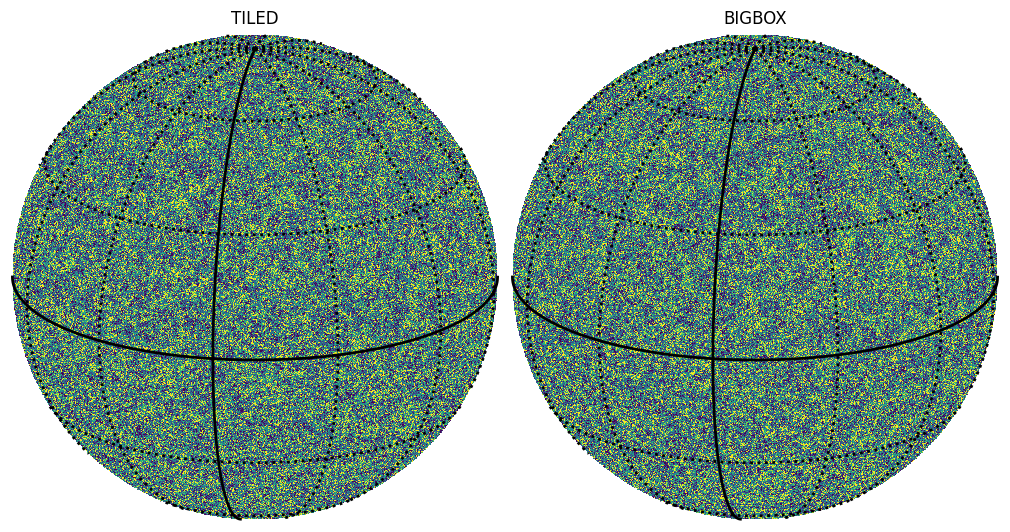
\includegraphics[width=\textwidth]{figures/samplemap.png}
    \caption[Convergence maps generated from the BIGBOX and TILED simulations]{Convergence maps generated from the BIGBOX and TILED simulations for source redshift $z_s = 1.5$. The yellow regions represent positive convergence, while the blue regions indicate negative convergence. The convergence maps exhibit similar large-scale structures.} \label{fig:convergence_maps}
\end{figure}

\section{Incorporating Galaxy Shape Noise into Convergence Maps}
In real observations, measurements of the lensing signal are contaminated by noise arising from the intrinsic shapes of galaxies and errors in shape measurements. This noise, referred to as shape noise, constitutes a significant source of uncertainty, particularly on small angular scales. For instance, 

We considered four different surveys with varying galaxy number densities, as detailed in Table~\ref{tab:survey_comparison}.
The variance of the shape noise per pixel was calculated as:
\begin{equation}
    \sigma_{\kappa, \text{noise}}^2 = \frac{\sigma_{\epsilon}^2}{2 n_{\mathrm{gal}} A_{\mathrm{pix}}},
\end{equation}
where $\sigma_{\epsilon}$ is the intrinsic ellipticity dispersion of galaxies, set to $\sigma_{\epsilon} = 0.26$ \citep{2019A&A...627A..59E}, $n_{\mathrm{gal}}$ is the galaxy number density per square arcminute, and $A_{\mathrm{pix}}$ is the solid angle of a pixel, set to $0.43$ arcminutes$^2$.
We generated a Gaussian random field $n(\hat{\mathbf{n}})$ with the calculated variance and added it to the convergence maps:
\begin{equation}
    \kappa_{\mathrm{obs}}(\hat{\mathbf{n}}) = \kappa(\hat{\mathbf{n}}) + n(\hat{\mathbf{n}}).
\end{equation}

\section{Patch Selection and Projection} \label{sec:patch_selection}
In order to simlplify the analysis onto a flat patch, we extracted $10^\circ \times 10^\circ$ patches from the full-sky convergence maps. In order to use the maximum number of uniformly distributed patches without repitition, we employed a Fibonacci grid \citep{2006QJRMS.132.1769S, 2023MNRAS.524.5591F} to extract patches from the full-sky map. The center of each patch is positioned at the vertices of the Fibonacci grid defined by golden ratio spirals:
\begin{equation}
    \sin \theta_i = \frac{2i}{2N + 1}, \quad \phi_i = \frac{2 \pi i}{\varphi}, \quad -N \leq i \leq N, \quad -\frac{\pi}{2} \leq \theta_i \leq \frac{\pi}{2},
\end{equation}
where $N$ is the number of patches and $\varphi = (1 + \sqrt{5})/2$ is the golden ratio. The visualization of the Fibonacci grid is shown in Figure~\ref{fig:fibonacci}.
\begin{figure}[ht]
    \centering
    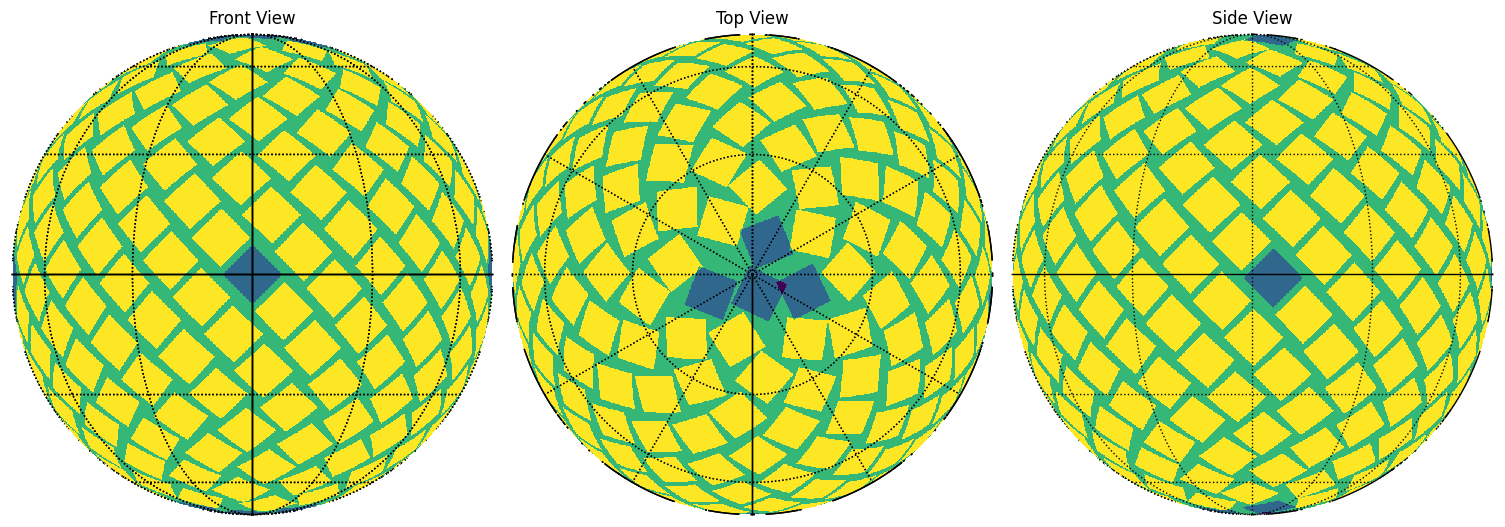
\includegraphics[width=\textwidth]{figures/fibonacci_grid.png}
    \caption[Visualization of the Fibonacci grids]{Visualization of the Fibonacci grid with $N_{\text{patches}} = 273$ patches, each covering approximately $10 \times 10$\,deg$^2$. 
    After the optimization and masking, the number of patches is reduced to $N_{\text{patches}} = 194$, effectively covering $47 \%$ of the sky.
    Each panel show the patches distribution on the Front, Top view and the final patches from the front.}\label{fig:fibonacci}
\end{figure}
Following \citet{2023MNRAS.524.5591F}, we can obtain the maximum number of patches by align the diagonal of square patches with the longitude lines. Nonetheless, we have to extract patches which their sides are aligned with the latitude lines due to the programming reason. Therefore, we first obtain a patch with wider side length and then rotate and crop the patch to get the desired shape.

Before extracting the patches, we first optimize the number of patches to extract from the full-sky map. The number of patches, denoted \( N_{\text{patches}} \), was optimized to ensure that individual patches do not overlap, except in regions near the poles where overlapping patches were subsequently discarded. 
Each patch on the full-sky map is defined as:
\begin{align}
    \left( \theta_i - R_{\text{patch}},\, \phi_i + R_{\text{patch}} \sin \theta_i \right),  \quad & \left( \theta_i + R_{\text{patch}},\, \phi_i + R_{\text{patch}} \sin \theta_i \right), \nonumber \\
    \left( \theta_i - R_{\text{patch}},\, \phi_i - R_{\text{patch}} \sin \theta_i \right), \quad &
    \left( \theta_i + R_{\text{patch}},\, \phi_i - R_{\text{patch}} \sin \theta_i \right)
\end{align}
with \( R_{\text{patch}} = 5\sqrt{2}\, \mathrm{\deg} \), the half diagonal length of the patch.
The optimization process commenced with an initial count of \( N_{\text{patches}} = 400 \) and involved iteratively reducing this number until a configuration was achieved wherein the patches remained non-overlapping, except for centers located within \( 2R_{\text{patch}}\) of the poles, that is $|\theta_i| \geq 2R_{\text{patch}}$ and $|\phi_i| \leq \pi - 2R_{\text{patch}}$. This threshold was selected to ensure that the patches were not including the poles.
After optimization and masking, the number of patches was set to $N_{\text{patches}} = 273$, effectively reducing to $N_{\text{patches}} = 265$, effectively cover $64 \%$ of the sky. Additionally, patches include points heavily tiled along with line of sight are excluded to avoid severe Box Replication Effect (see Sec.~\ref{sec:boxreplication} for further check). Hence, the final number of patches used for analysis is $N_{\text{patches}} = 194$, covering $47 \%$ of the sky.

For a Fibonacci grid center characterized by coordinates \( (\theta_i, \phi_i) \), we first employed the \texttt{gnomview} function from the \texttt{healpy} library \citep{Zonca2019} to project each spherical patch onto a flat plane via a gnomonic projection. Then for each patch, we rotated them by $45^\circ$ around the center of the patch to align the diagonal of the patch with the longitude lines. Finally, we cropped the patch according to the corresponding vertices. Figure~\ref{fig:fibonacci_extraction} showcases an extracted patch from the full-sky convergence map, and additional handling of the patches to get the desireed shape.
\begin{figure}
    \centering
    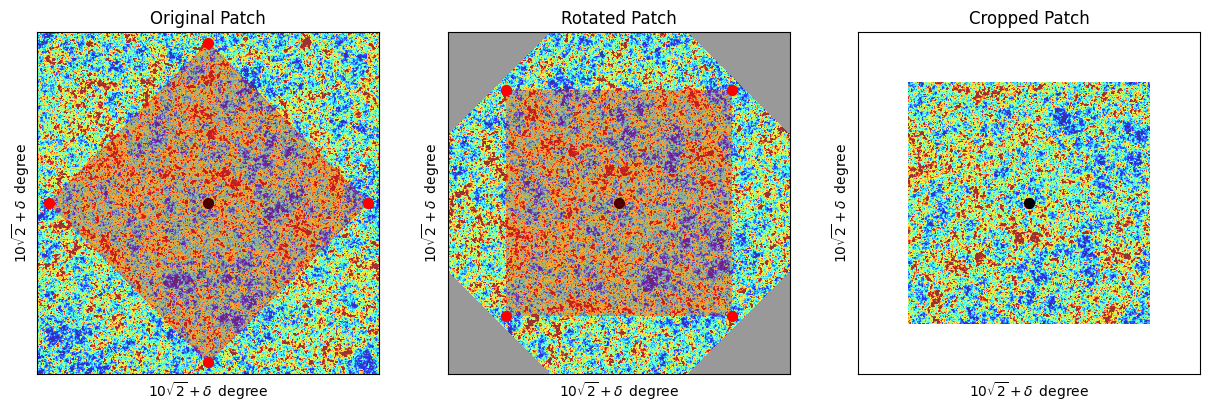
\includegraphics[width=\textwidth]{figures/fibonacci_extraction.png}
    \caption[Extraction of a patch from the full-sky convergence map using a Fibonacci grid]{Extraction of a patch from the full-sky convergence map using a Fibonacci grid. The patch covers an area of $10^\circ \times 10^\circ$ and is centered at the vertices of the Fibonacci grid. From the left to the right, the panels show the original extracted patch, patch rotated $45^\circ$ around the center and the final patch after the second rotation. The red shaded region represents the final patch we used for analysis.
    } \label{fig:fibonacci_extraction}
\end{figure}

Each patch is represented by a $2048 \times 2048$ grid of pixels, resulting in a pixel size of:
\begin{equation}
    \Delta \theta = \frac{10^\circ}{2048} \approx 0.00488^\circ \approx 0.293' \quad \text{per pixel}.
\end{equation}
For each realization, the covariance is computed using 194 patches extracted from the full-sky map of each simulation.
Therefore, we obtain a total of 2134 patches from the BIGBOX simulation and 3880 patches from the TILED simulation. This ensemble of patches allows us to robustly sample cosmic variance and shot noise, ensuring that our statistical analyses are at least sufficient for the power spectrum at $\ell = 5283$ and peak counts in $ \kappa \in \left[-0.06, 0.45\right]$ \citep{2016PhRvD..93f3524P}.

\section{Applying Gaussian Kernels to Convergence Fields}
Shape noise predominantly affects small angular scales. To mitigate this noise and enhance the detection of the underlying lensing signal, we applied Gaussian smoothing to the noisy convergence maps. The Gaussian filter used is defined by:
\begin{equation}
    W(\theta) = \frac{1}{\pi \theta_{\mathrm{G}}^2} \exp\left( -\frac{\theta^2}{\theta_{\mathrm{G}}^2} \right),
\end{equation}
where $\theta$ is the angular distance from the center of the filter, and $\theta_{\mathrm{G}}$ is the smoothing scale. For our analysis, we selected $\theta_{\mathrm{G}} = 2'$, $5'$, $8'$, and $10'$.

By convolving the noisy convergence map with the Gaussian filter, we obtained the smoothed convergence map:
\begin{equation}
    \kappa_{\mathrm{smoothed}}(\hat{\mathbf{n}}) = \int d\Omega' \, W(|\hat{\mathbf{n}} - \hat{\mathbf{n}}'|) \kappa_{\mathrm{obs}}(\hat{\mathbf{n}}').
\end{equation}

Figure~\ref{fig:smoothing} illustrates the impact of Gaussian smoothing on a noisy convergence map, highlighting the progressive suppression of small-scale fluctuations. The figure comprises four panels, each corresponding to a distinct smoothing scale: $\theta_{\mathrm{G}} = 2'$, $5'$, $8'$, and $10'$. As the smoothing scale is increased, convolution with the Gaussian kernel increasingly attenuates small-scale noise, thereby reducing the amplitude of small-scale fluctuations in the map. While this process naturally diminishes the power spectrum at small angular scales, a smoothing scale lower than $10'$ proves adequate to mitigate the influence of shape noise, still retains the non-Gaussian structures in the convergence field.
\begin{figure}[ht]
    \centering
    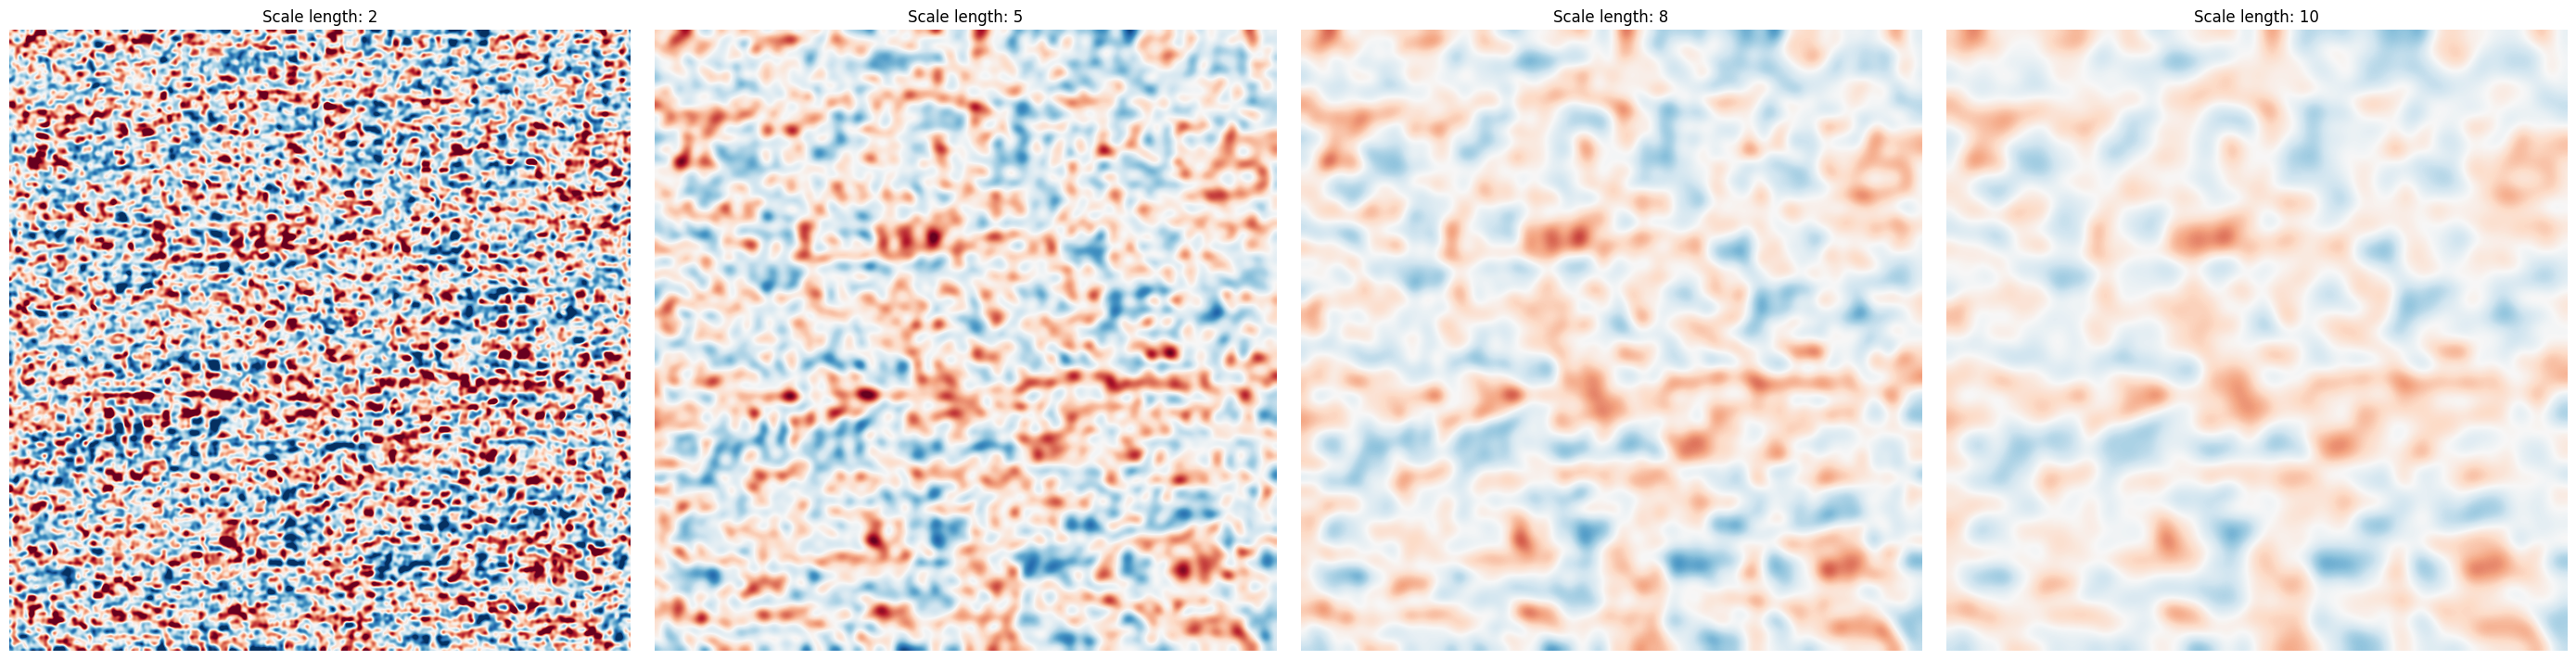
\includegraphics[width=\textwidth]{figures/smoothed_comparison.png}
    \caption[Gaussian smoothing on a noisy convergence map for multiple smoothing scales]{Effect of Gaussian smoothing on a noisy convergence map. Each panel shows the result of applying a Gaussian filter with a different smoothing scale $\theta_{\mathrm{G}} = 2'$, $5'$, $8'$, and $10'$. As the smoothing scale increases, small-scale noise is progressively suppressed, and large-scale structures become more prominent. This demonstrates how Gaussian smoothing effectively reduces shape noise while enhancing the detection of the underlying lensing signal.}
\label{fig:smoothing}
\end{figure}

For the analysis of non-Gaussian statistics, we employ a Gaussian smoothing procedure, after which the statistics are computed from the resulting smoothed convergence maps. The application of a smoothing kernel effectively suppresses small-scale structures, thereby modifying the range of $\kappa$ values. To avoid the smoothing issues and the complex binning to consider, we normalize $\kappa$ values by the standard deviation of each patch's convergence map, $\sigma_{\kappa}$. 

Figure~\ref{fig:avg_sigma0} presents the mean standard deviation of the noiseless convergence maps obtained from both the BIGBOX and TILED simulations. There is no significant difference between the two simulations, but the standard deviation increases with redshift and smoothing scale. The observed trend with respect to redshift reflects the inclusion of additional shells along the line of sight and the resulting greater variability in density contrasts. In parallel, the trend with respect to the smoothing scale emerges from the nature of the smoothing process itself, which suppresses small-scale structures and consequently broadens the distribution of larger-scale fluctuations.

\begin{figure}[ht]
    \centering
    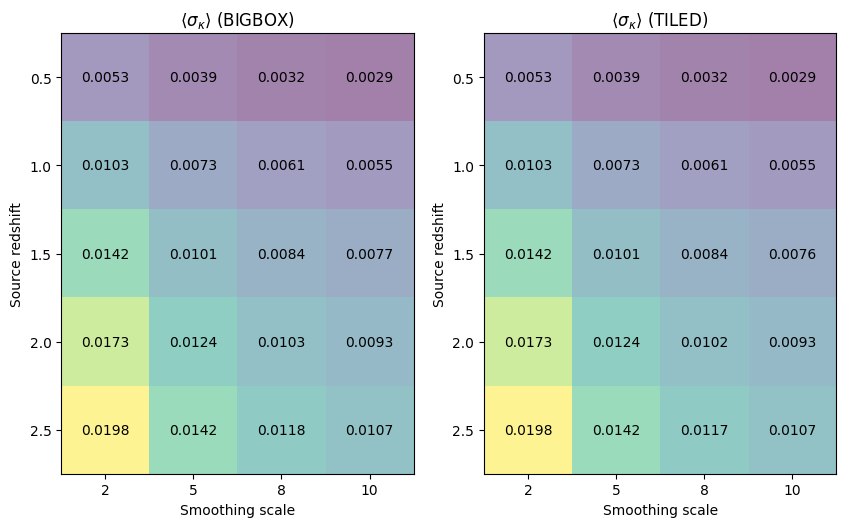
\includegraphics[width=\textwidth]{figures/avg_sigma0.png}
    \caption[Average standard deviation of the noiseless convergence maps]{Average standard deviation of the noiseless convergence maps for the BIGBOX and TILED simulations. The standard deviation increases with redshift and smoothing scale, with a subtle difference between the BIGBOX and TILED simulations.} \label{fig:avg_sigma0}
\end{figure}

\section{Extracting Weak Lensing Statistics from Convergence Maps}
In order to characterize the influence of super-sample covariance on higher-order statistics, this study concentrates on the bispectrum, probability distribution function (PDF), peak counts, minima counts, and Minkowski functionals. 

Table~\ref{tab:statistics} delineates the range of values and the computational subroutines employed for each statistical measure. 
\begin{table*}[htbp]
    \centering
    \begin{tabular}{lcc}
    \toprule
    \textbf{Statistic} & \textbf{Range} & \textbf{Subroutine (Sky Patch)} \\
    \midrule
    Angular Power Spectrum & $300 \leq \ell \leq 3000$ & \texttt{lenstools.powerSpectrum} \\
    Bispectrum & $300 \leq \ell \leq 3000$ & \texttt{lenstools.bispectrum} \\
    Peak Counts & $-4 \leq \kappa/\sigma_\kappa \leq 4$ & \texttt{lenstools.peakCount} \\
    Minima Counts & $-4 \leq \kappa/\sigma_\kappa \leq 4$ & \texttt{lenstools.peakCount} \\
    Probability Distribution Function (PDF) & $-4 \leq \kappa/\sigma_\kappa \leq 4$ & \texttt{lenstools.pdf} \\
    Minkowski Functionals & $-4 \leq \kappa/\sigma_\kappa \leq 4$ & own implementation \\
    \bottomrule
    \end{tabular}
    \caption{Summary of the statistical measures employed in this investigation, including their respective value ranges and computational subroutines utilized for analyses.}\label{tab:statistics}
\end{table*}

\subsection{Angular Power Spectrum}
The angular power spectrum ($C_{\ell}^{\kappa\kappa}$) is estimated directly from the simulated convergence maps using \texttt{lenstools} \citep{2016A&C....17...73P}, without any preliminary smoothing. The multipole range considered spans from $\ell = 300$ to $\ell = 3000$, partitioned into $8$ logarithmically spaced bins. This binning scheme is chosen to maintain consistency with the multipole selection employed in the Hyper Suprime-Cam Year 3 (HSC Y3) cosmic shear analysis \citep{2023PhRvD.108l3519D}. The lower limit of $\ell = 300$ is selected to exclude large-scale modes, as the primary focus of this study is on investigating higher-order statistics, which are most sensitive to intermediate and small angular scales. Conversely, the upper limit of $\ell = 3000$ ensures that our analysis incorporates sufficiently small-scale modes, where the super-sample effect becomes increasingly pronounced. Moreover, this chosen multipole range is robust for the number of sampling of simulated maps, as discussed in Section~\ref{sec:patch_selection}.

For benchmarking purposes, we compute the theoretical angular power spectrum prediction using the \texttt{Halofit} model \citep{2012ApJ...761..152T} and compare it with the measured angular power spectrum. 
The theoretical prediction is generated using an identical set of cosmological parameters as those employed in the simulations.

\subsection{Bispectrum}
The bispectrum ($B_{\ell}$) is computed from the unsmoothed convergence maps using \texttt{lenstools}. We consider three distinct configurations: equilateral ($\ell_1 = \ell_2 = \ell_3$), squeezed ($\ell_1 = \ell_2 = 10\ell_3$), and isosceles ($\ell_1 = \ell_2 = 2\ell_3$). 
Those configurations are chosen to capture the different shapes of the bispectrum and provide complementary information about the underlying matter distribution.
The bispectrum computations are confined within the same multipole range as the angular power spectrum, specifically $\ell \in [300, 3000]$, and are divided into $8$ logarithmically spaced bins. Though the bispectrum is more senstive to the noise and the small-scale structures, we maintain an identical multipole range facilitates a direct comparison with the angular power spectrum results

For theoretical validation, we compute the bispectrum prediction using the \texttt{BiHalofit} model \citep{2020ApJ...895..113T} and compare it against the measured bispectrum from the simulations. The theoretical bispectrum is derived using the same cosmological parameters as those utilized in the simulations.

\subsection{PDF}
We compute the probability distribution function (PDF) of the convergence field using \texttt{lenstools}. Each PDF is derived from the smoothed convergence maps over a normalized range of $-4 \leq \kappa/\sigma_{\kappa} \leq 4$, divided into 8 equally spaced bins. Here, $\sigma_{\kappa}$ represents the standard deviation of the convergence field within each individual patch. The range is chosen to match the study of \citet{2023arXiv230405928T}, but the binning is optimized to ensure that each bin contains a sufficient number of data points.

The theoretical prediction for the PDF is obtained using the \texttt{hmpdf} code \citep{2020PhRvD.102l3545T}, employing the same linear matter power spectrum as used in the simulations. We subsequently compare the theoretically predicted PDF with the measured PDF to assess the consistency and accuracy of the underlying cosmological model and related assumptions.

\subsection{Peak/Minima Counts}
Peak and minima counts are likewise computed from the smoothed convergence maps using \texttt{lenstools} and performed over the same normalized range as the PDF, namely $-4 \leq \kappa/\sigma_{\kappa} \leq 4$, with 8 evenly spaced bins. Although the highest and lowest peaks are represented by relatively few data points, we retain these extreme bins to maintain consistency with the binning scheme adopted for the PDF.

\subsection{Minkowski Functionals}
The Minkowski functionals are calculated from the smoothed convergence maps using a custom implementation that closely follows the definitions presented in Section~\ref{sec:minkowski_functionals}. As with the PDF and peak/minima counts, these functionals are computed over the normalized range $-4 \leq \kappa/\sigma_{\kappa} \leq 4$, divided into 8 linearly spaced bins. 

Figure~\ref{fig:avg_sigma1} illustrates the variance of the gradient field, $\sigma_1 = \sqrt{\kappa_x^2 + \kappa_y^2}$, which is an essential input for calculating the Minkowski functionals. As the smoothing scale increases, the values of $\sigma_1$ decrease, reflecting the diminished influence of small-scale structures. Differences between the BIGBOX and TILED simulations, as well as across varying redshifts, remain subtle, underscoring the robustness of these measures and their relative insensitivity to large-scale environmental differences.

\begin{figure}[ht]
    \centering
    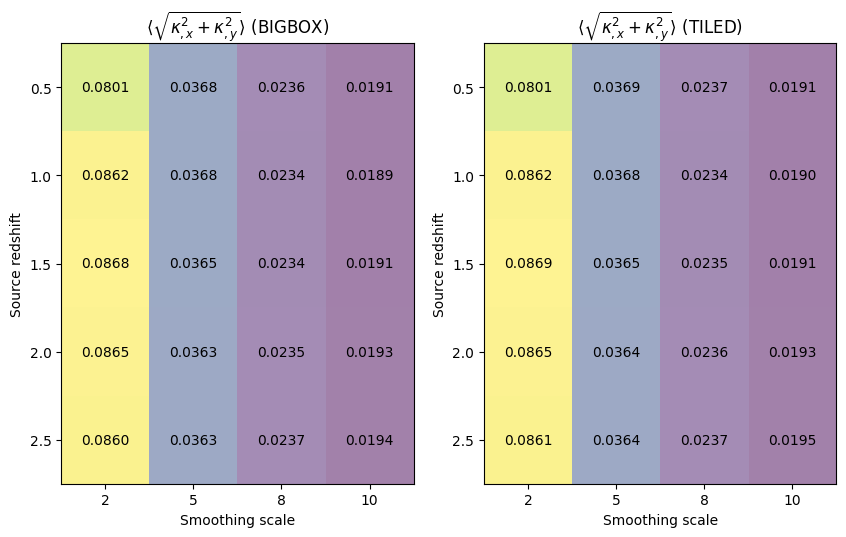
\includegraphics[width=\textwidth]{figures/avg_sigma1.png}
    \caption[Average $\sigma_1 = \sqrt{\kappa_{x}^2 + \kappa_{y}^2}$ of the noiseless convergence maps]{Average $\sigma_1 = \sqrt{\kappa_{x}^2 + \kappa_{y}^2}$ of the noiseless convergence maps for the BIGBOX and TILED simulations. They are calculated for the smoothing scales $\theta_{\mathrm{G}} = 2'$, $5'$, $8'$, and $10'$. The values decrease as the smoothing scale increases, while the difference between the BIGBOX and TILED simulations or the redshifts is subtle.
    } \label{fig:avg_sigma1}
\end{figure}

\section{Comparing Covariances from BIGBOX and TILED}
Following the measurement phase, this study examines the influence of super-sample covariance on the covariance matrices associated with the aforementioned statistical measures. To achieve this, we employ an unbiased estimator for the covariance matrix as previously defined in Equation~\ref{eq:covariance}. 
\begin{equation}
    \label{eq:covariance}
    \mathrm{Cov}(\mathcal{O}_i, \mathcal{O}_j) = \frac{1}{N_{\mathrm{sim}} - 1} \sum_{n=1}^{N_{\mathrm{sim}}} (\mathcal{O}_i^{(n)} - \langle \mathcal{O}_i \rangle) (\mathcal{O}_j^{(n)} - \langle \mathcal{O}_j \rangle),
\end{equation}

Additionally, we also compute the correlation matrix for each statistical measure to investigate the interdependence between different scales and configurations. The correlation matrix is defined as:
\begin{equation}
    \rho_{ij} = \frac{\text{Cov}(\mathcal{O}_i, \mathcal{O}_j)}{\sqrt{\text{Cov}(\mathcal{O}_i, \mathcal{O}_i)\text{Cov}(\mathcal{O}_j, \mathcal{O}_j)}},
\end{equation}
where $\mathcal{O}_i$ and $\mathcal{O}_j$ represent the $i$-th and $j$-th statistical measures, respectively. Correlation matrix normalize off-diagonal elements by the scale dependent variance, thereby enabling a direct comparison between different simulations and statistical measures.

Once both the BIGBOX and TILED simulations have been used to compute the corresponding covariance and correlation matrices, we proceed to assess the impact of super-sample covariance by comparing these two sets of matrices. The comparison is performed by taking the ratio of the BIGBOX to TILED matrices, defined as:
\begin{equation}
    R^{\mathrm{Cov}}_{ij} = \frac{\mathrm{Cov}^{\mathrm{BIGBOX}}_{ij}}{\mathrm{Cov}^{\mathrm{TILED}}_{ij}}, \quad R^{\rho}_{ij} = \frac{\rho^{\mathrm{BIGBOX}}_{ij}}{\rho^{\mathrm{TILED}}_{ij}},
\end{equation}
where $\mathrm{Cov}_{\mathrm{BIGBOX}}$ and $\mathrm{Cov}_{\mathrm{TILED}}$ denote the covariance matrices derived from the BIGBOX and TILED simulations, respectively. Similarly, $\rho_{\mathrm{BIGBOX}}$ and $\rho_{\mathrm{TILED}}$ represent the corresponding correlation matrices.

To quantitatively evaluate the overall influence of super-sample covariance, we compute the mean values of the ratios $R^{\mathrm{Cov}}_{ij}$ and $R^{\rho}_{ij}$ across the respective covariance and correlation matrices. Specifically, the average of $R^{\rho}$ is calculated by excluding the diagonal elements, which are intrinsically equal to unity by definition. In contrast, the average of $R^{\mathrm{Cov}}$ utilizes all elements of the covariance matrix, including the diagonal. For $\ell$-binned statistics, such as the angular power spectrum ($C_\ell^{\kappa\kappa}$) and the bispectrum, the average ratio is determined across all available multipole bins. Conversely, for $\nu$-binned statistics, such as the PDF, peak/minima counts, and Minkowski functionals, the first and last bins are excluded from the ratio calculation. This exclusion is necessary to avoid biases introduced by limited data points and the inherent unreliability of these extreme bins. In equation form, the average ratios are defined as:
\begin{equation}
    \langle R^{\mathrm{Cov}} \rangle = \frac{1}{N_{\mathrm{bins}}^2} \sum_{i, j} R^{\mathrm{Cov}}_{ij}, \quad \langle R^{\rho} \rangle = \frac{1}{N_{\mathrm{bins}}^2 - N_{\mathrm{bins}}} \sum_{i \neq j} R^{\rho}_{ij},
\end{equation}
where $N_{\mathrm{bins}} = 8$ for $\ell$-binned statistics and $N_{\mathrm{bins}} = 6$ for $\nu$-binned statistics.